%
% File acl2018.tex
%
%% Based on the style files for ACL-2017, with some changes, which were, in turn,
%% Based on the style files for ACL-2015, with some improvements
%%  taken from the NAACL-2016 style
%% Based on the style files for ACL-2014, which were, in turn,
%% based on ACL-2013, ACL-2012, ACL-2011, ACL-2010, ACL-IJCNLP-2009,
%% EACL-2009, IJCNLP-2008...
%% Based on the style files for EACL 2006 by
%%e.agirre@ehu.es or Sergi.Balari@uab.es
%% and that of ACL 08 by Joakim Nivre and Noah Smith

\documentclass[11pt,a4paper]{article}
\usepackage[hyperref]{acl2018}
\usepackage{times}
\usepackage{latexsym}
\usepackage{graphicx}

\usepackage{url}

\aclfinalcopy % Uncomment this line for the final submission
%\def\aclpaperid{***} %  Enter the acl Paper ID here

%\setlength\titlebox{5cm}
% You can expand the titlebox if you need extra space
% to show all the authors. Please do not make the titlebox
% smaller than 5cm (the original size); we will check this
% in the camera-ready version and ask you to change it back.

\newcommand\BibTeX{B{\sc ib}\TeX}

\title{Graph Models of Named Entity Types\\for Interpretable Named Entity Recognition}

\author{Andrew Larimer \\
  {\tt andrewlarimer@berkeley.edu} \\\And
  Daniel Rasband \\
  {\tt danrasband@berkeley.edu} \\}
  
\date{12/07/18}

\begin{document}
\maketitle
\begin{abstract}
Like many neural networks, the decisions made by most Named Entity Recognition systems are difficult to interpret or adjust. We prototype a new Named Entity Recognition architecture that is very transparent and could be manually adjusted. Additionally, it is syntactically aware and focuses only on words with a direct dependency relationship to the entity in question, filtering out the noise of nearby words. Finally, our system builds a clear and cumulative 'mental model' of each named entity type, which may be extensible as a structure for persistent knowledge across long texts or for longterm knowledge-building.
\end{abstract}

\section{Introduction}

Named Entity Recognition systems continue to improve, but state-of-the-art accuracy is still below 90\% on popular benchmarks like the OntoNotes 5.0 corpus.

Errors at this task can be particularly frustrating, as the fact that a given person in a text is, in fact, a person can seem obvious to a human reader, and we can confidently point to specific elements in the text that indicate as such, but due to the oft-bemoaned black-boxiness of neural networks, we have no way of directly communicating that knowledge to current state-of-the-art systems.

These systems also don't provide a clear view of exactly what a neural network considers a PERSON to be in comparison with an ORGANISATION, or why a given tag was assigned. By contrast, we can at least explore word embeddings in comparison to one another, but current NER systems don't provide us an easy way to compare internal representations of different entity types.

To solve these problems, we propose a system of clear 'mental models' of each Named Entity type labeled in the OntoNotes corpus, constructed as a grammar-aware graph from labeled data. Figure \ref{fig:person_graph} shows an example of a dramatically pruned version of our representation of the PERSON entity type. By 'grammar-aware', we mean that each Named Entity type has a subgraph corresponding to how the entity is used in that sentence. In Figure  \ref{fig:person_graph}, we see that when a PERSON is the subject of a verb with an active tense, they might concede, dare, or sign. When they are a direct object, someone or something might be urging them, bringing them, or handing them something. If used as a possession modifier, a person might have a widow, a son, or words.

\begin{figure}[h]
  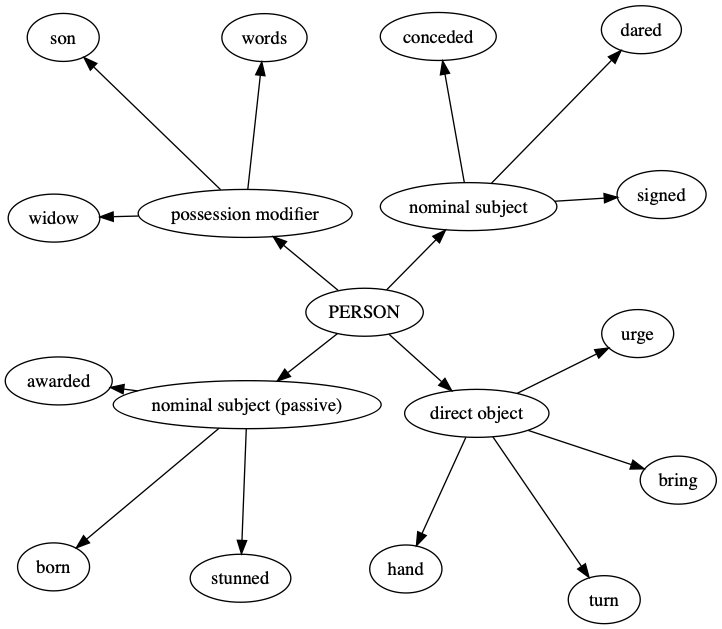
\includegraphics[width=\linewidth]{figures/G_PERSON.png}
  \caption{A simplified version of a Named Entity Type graph.}
  \label{fig:person_graph}
\end{figure}

When conducting inference, we currently receive named entity candidates from an existing named entity system. Then to classify that candidate, we construct a graph for it based on its ancestor and child dependency tags, as well those dependency tags of coreferences to that entity. We compare that candidate graph against our entity template graphs through a similarity measure we have developed, and choose the label with the greatest similarity. By focusing on syntactic subgraphs depending on how the entity is used within the sentence, we are able to reduce computation time required to process each entity, as well as focus on subtle differences in what various entity types do or have done to them.

While building these 'mental models' from a dependency parse, the strength of this construct is that it is cumulative, and by including coreferences we can develop a more complete understanding of an entity before attempting to classify it.

As alluded to earlier, our model is also transparent and easily adjusted. In the event of errors within a particular domain, a user could prune the leaf nodes causing confusion or add in additional leaf nodes to help better identify entities within their field.

We envision this system developing into a powerful classifier for longer literary works such as novels, particularly as we develop more fine-grained named entity types. With additional refinement and the appropriate labeled dataset, we could classify a protagonist in a novel as a traditional hero or an anti-hero. We could identify occupations and/or literary tropes represented by supporting characters. And interesting tools for authors or publishers could be developed by tracking changes in a character's behavior from heroic to antiheroic from chapter to chapter.

Furthermore, we see the potential of graph-based 'mental constructs' as having additional applications in the progression of machine learning. We believe transition-based parsing approaches could directly build on these graphs, and logical operations could be conducted on them to build out unstated but implied nodes that enhance our understanding of entities beyond what is explicitly stated.

\section{Background}

We will flesh out this section, but we considered several papers, including:
\begin{itemize}
\item Interleaving Ontology-Based Reasoning and Natural Language Processing for Character Identification in Folktales. Suciu et al.

\item Fast and Accurate Entity Recognition with Iterated Dilated Convolutions. Strubell et al.

\item Algorithms for Graph Similarity and Subgraph Matching. Koutra et al.

\item Neural Architectures for Named Entity Recognition. Lample et al.

While the field of Question Answering is distinct from NER, we were additionally inspired by the "propose candidates and double-check them" approach of this "Read + Verify" approach to Squad 2.0:

\item Read + Verify: Machine Reading Comprehension with Unanswerable Questions. Hu et al.
\end{itemize}

\section{Methods}

We use the OntoNotes 5.0 corpus for its 143,709 sentences with labeled named entities.

\subsection{Creating our Named Entity Type 'Mental Constructs'}

For each occurrence of a labeled named entity in that corpus, we do the following:

1. If this occurrence of a named entity consists of more than one word (ex. 'Nobel Peace Prize'), we assume the head of the phrase to be the last word of the named entity phrase.

2. We load the graph for the Named Entity Type represented by that occurrence (PERSON, ORGANIZATION, WORK OF ART, etc.).

3. We check to see if that Named Entity Type graph already has a child node corresponding to the dependency tag of the head of our named entity phrase. We call these nodes "syntactic function nodes."  In the 'Nobel Peace Prize' example, we see that 'Prize' is a 'direct object', so we find the 'direct object' child node of our 'WORK OF ART' entity type node. If there isn't already that child node, we create it. If it is already there, we increase a score count by one for the sake of generating weights later on.

4. Under the appropriate "intermediary grammar node," we add a leaf node for our named entity's head in the dependency parse. In the "Nobel Peace Prize" example, the head of "Prize" when it was used as a direct object is "awarded," so we create a node for "awarded" as a child node of "direct object" and give it a score of one, unless it already exists, in which case we increase its score by one.

5. For the special case of arriving at a preposition, we take an extra arc to find the word that is that preposition's head, as we found more signal present in those head words than in the prepositions themselves.

6. After running through the corpus and building the graphs, we divide the score of each "syntactic function node" by the total occurrences of the named entity type to have weights between 0 and 1. We also normalize each leaf token's weight by dividing by its parent "syntactic function node"'s count, to also result in a weight from 0 to 1.

\subsection{Conducting Inference on a New Named Entity Candidate}

We consider each Named Entity as identified by an existing NER system (spaCy's built-in NER system) as a candidate, and do the following:

1. We construct a candidate graph in a similar manner to the one described above for generating the Named Entity Type (NET) graphs. We use a coreference system to include multiple references to the entity in order to have as robust a graph as possible to compare against our NET graphs.

2. We compare our candidate graph to each of the eighteen Named Entity Type graphs. For each leaf node in our candidate graph, we get its "syntactic function node", and so we focus our search on the child nodes of the Named Entity Type's corresponding syntactic function.

3. For each child node of that corresponding "syntactic function node," we calculate a score as follows: the similarity of the two words' embeddings (according to spaCy's Token.similarity() method, which is presumably a cosine similarity of the vectors but is not explicitly stated as such in their documentation) is multiplied by the weight of that leaf node in the Named Entity Type graph (which we calculated above based on its frequency of use within that grammatical context). By using the cosine similarity of the embeddings, we are more capable of performing inference on new candidate words that we don't find in any given Named Entity Type graph, but which may be similar. We are still considering how we will score a candidate word for which we don't have an embedding.

4. We sum the scores of each "syntactic function node"'s highest-scoring child node to arrive at the similarity score for that Named Entity Type Graph.

5. We compare the score of each NET graph, and choose the highest-scoring type which best matched our candidate graph as our prediction.


\section{Results and discussion}

We will develop our model on a dev set, and test our prediction accuracy against the labels in a held-out test set from the OntoNotes 5.0 corpus.

We will compare our performance against a baseline of the built-in spaCy NER module, which we will run on the same test set. Its performance is similar to other state of the art named entity recognition models, as seen in Figure \ref{fig:state_of_art}.

\begin{figure}[h]
  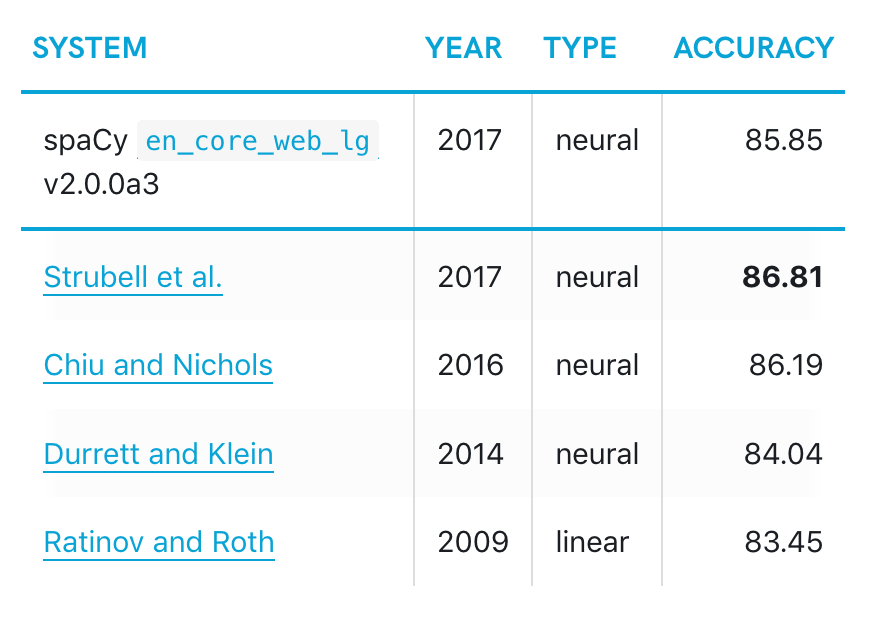
\includegraphics[width=\linewidth]{figures/state_of_art_spaCy.png}
  \caption{Scores of state of the art models on the OntoNotes 5.0 corpus.}
  \label{fig:state_of_art}
\end{figure}

\section{Next Steps}

We anticipate finishing our code for the above model in the next day or two, and then evaluating whether we have time to add possible enhancements.

Ideas for possible enhancements include:

\begin{itemize}

\item If it appears we are filtering out too much signal by being too selective, we are considering adding a hyperparameter that would not just take the immediate head and children of each entity in our NET graphs and inference candidates, but take one or two additional generations of head and child nodes, if they exist. This might allow us to take in more information while still filtering out noise that doesn't have a directly traceable dependency relation to the entity in question.

\item If inference is too slow due to the large size of the NET graphs, we have considered compressing the information in those graphs by clustering the leaf nodes using a Partitioning Around Medoids algorithm to find the 50 or so most representative leaf nodes and having those absorb the weights of the other members in their cluster, which we could then discard. We think this serve as a sort of regularization to allow the model to accept more synonyms rather than exact matches of candidates entity's heads to leaf nodes, while still maintaining the clarity of having real word leaf nodes.

\item Alternatively, if the model is too sensitive to whether a candidate entity's head matches exactly to a leaf node in our NET graphs, we could do clustering of the leaf node words via k-means, such that our clusters' centers would \textit{not} be actual words, but would exist somewhere in the embedding space near the words, and thus no word would likely be a 100\% match. To maintain interpretability, we could maintain a list of the closest leaf node to each cluster center.

\item We considered giving each syntactic function node a trainable weight, and then training those weights via a logistic regression type neural network to emphasize or deemphasize the importance of certain syntactic functions for classifying certain Named Entity Types, but we don't expect the candidate graphs to have enough different syntactic functions represented to make this worthwhile.

\item We are considering pruning stop words from the NET graphs, or using TF-IDF to dampen the weights of common words that might be found on several NET graphs (defining the graphs as the documents for purposes of the IDF).

\end{itemize}


%Citation Example: Papantoniou \shortcite{Pap:2016}

\bibliographystyle{acl_natbib}
\bibliography{LarimerRasbandW266FinalProject2018}

\end{document}
